O projeto foi desenvolvido com React, para criar interfaces de usuário dinâmicas, e Node.js, que permite executar JavaScript no servidor. Para o back-end, foram utilizadas dependências como Express, para gerenciar rotas e APIs; Cors, para controlar o acesso entre diferentes origens; JWT, para autenticação; e Mongoose, para modelagem e manipulação de dados no MongoDB, um banco de dados NoSQL que permite armazenar informações de forma flexível e escalável. 

O MongoDB foi hospedado no MongoAtlas, plataforma na nuvem que facilita a gestão, segurança e escalabilidade do banco, enquanto o back-end e a API estão no Render, serviço de nuvem para aplicações web, e o front-end no Vercel, plataforma otimizada para deploy rápido e escalável de aplicações web. O sistema foi projetado para uso em dispositivos móveis, oferecendo maior praticidade para o usuário no dia a dia, sendo desenvolvido como Aplicativo Web Progressivo (do inglês, Progressive Web App, ou PWA), que permite que a aplicação funcione como um app nativo, instalação na tela inicial e desempenho otimizado mesmo em navegadores web. 

\section*{Funcionamento do projeto}

No fluxograma apresentado abaixo, é descrito o funcionamento geral do projeto. Na Figura 1, o usuário realiza o cadastro no aplicativo e solicita o cadastramento do cativeiro, necessário para que a equipe responsável realize a instalação dos equipamentos IoT no local.

Na Figura 2, após a autorização do cadastro do cativeiro, o usuário pode acessar todas as informações referentes aos cativeiros, de forma geral ou individual, por meio de um dashboard.

Na Figura 3, todos os dados inseridos na aplicação são enviados para o banco de dados, que armazena as informações e as disponibiliza para visualização pelo usuário. Além disso, o banco de dados envia os dados coletados para o equipamento IoT, conforme mostrado na Figura 4.

Na Figura 4, o equipamento IoT, representado pelo ESP32, utiliza seus sensores de temperatura, pH e amônia para captar os dados do cativeiro e enviá-los ao banco de dados, garantindo que o usuário tenha acesso às informações coletadas em tempo real.

Na Figura 5, os dados enviados do banco de dados também são encaminhados para o dispensador de ração, contendo informações sobre o horário e a quantidade de alimento. O dispenser armazena essas instruções e realiza a alimentação no momento programado pelo usuário. Após a alimentação, um alerta é enviado ao aplicativo, informando que o procedimento foi realizado com sucesso.

\begin{figure}[!htb]
\SetCaptionWidth{\ifbool{@LayoutA}{0.7}{0.72}\linewidth}
\caption{Fluxograma sobre funcionamento do sistema}%
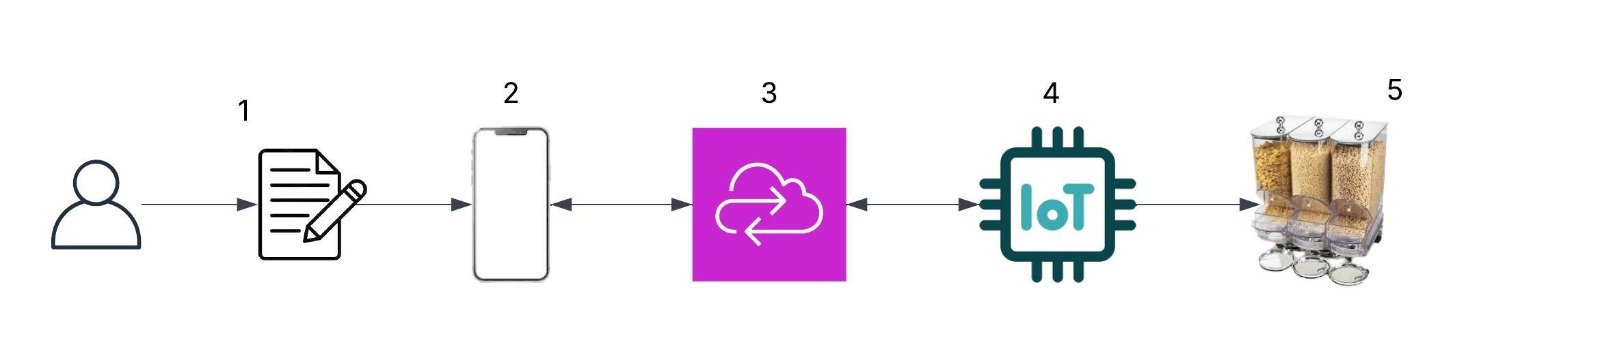
\includegraphics[width = 1.55\CaptionWidth]{Imagem/Fluxograma.jpeg}
\SourceOrNote{Autoria Própria}
\end{figure}